\documentclass[12pt]{article}
\usepackage[utf8]{inputenc}
\usepackage{amsmath, amssymb}
\usepackage{graphicx}
\usepackage{caption}
\usepackage{hyperref}
\usepackage{geometry}
\usepackage{cite}
\usepackage{relsize}

\usepackage{algpseudocode}
\usepackage{amsmath}
\usepackage{mathtools}
\usepackage[ruled,linesnumbered]{algorithm2e}

\geometry{margin=1in}

\begin{document}

\begin{center}
    {\LARGE \textbf{ANS for Solid-Beam Elements}}\\[0.5em]
    {\large Derivation and Implementation}\\[1em]
    \href{https://github.com/jaafaralaswad/Improved-Brick-Finite-Elements-for-Beam-Problems}{\texttt{github.com/jaafaralaswad/Improved-Brick-Finite-Elements-for-Beam-Problems}}\\[1em]
    \textit{Last updated: \today}
\end{center}
\vspace{2em}

We adopt the \textit{Assumed Natural Strain} (ANS) method as outlined in:

\begin{quote}
J.F.~Caseiro, R.F.~Valente, A.~Reali, J.~Kiendl, F.~Auricchio, and R.~Alves de Sousa,\\
\textit{On the Assumed Natural Strain method to alleviate locking in solid-shell NURBS-based finite elements},\\
\textit{Computational Mechanics}, \textbf{53}, 1341–1353 (2014).
\end{quote}

However, we adapt the formulation for beam problems, replace NURBS with Lagrange polynomials, and extend it to geometrically nonlinear analyses.


\tableofcontents
\bigskip
\hrule
\bigskip


\section{Assumed Natural Strain Method (ANS)}

The assumed natural strain method (ANS) was applied for the first time for Reissner–Mindlin plates and then was applied to shells. The method is developed to alleviate transverse shear, membrane and curvature-thickness locking.

A compatible strain component, $E^c$, which follows from geometrically nonlinear theory, can be calculated for any given point in the parametric domain, $(\xi, \eta, \zeta) \in \Omega_{\square}$, by:

\begin{equation}
E^c (\xi, \eta, \zeta) = \sum_{I=1}^{n_e} \tilde{\mathbf{B}}^e_I (\xi, \eta, \zeta) \mathbf{u}_I,
\end{equation}

\noindent
where $\tilde{\text{\bf{B}}}^e_I$, which has the dimensions $1 \times 3$, is the respective row of the standard compatible strain-displacement matrix, $\text{\bf{B}}^e_I$ , for the $e^{\text{th}}$ element evaluated at node $I$, $\text{\bf{u}}_I$ is the nodal displacements vector, of dimensions $3 \times 1$, at node $I$ and $n_e$ is the number of nodes in the element. The standard compatible strain-displacement matrix, $\text{\bf{B}}^e$, is constructed with the help of the shape functions that are used to interpolate the displacements, $N_I$.

The central idea in ANS method lies in interpolating the strains causing locking at so-called tying points, these strains will replace, in a weighted manner, the standard strain values calculated at the integration points. Thus, a strain component based on ANS method, $E^{\text{ANS}}$, evaluated at an integration point, $(\xi_{GP}, \eta_{GP}, \zeta_{GP})$, is obtained by interpolating the compatible strain values at the associated tying points, as follows:

\begin{equation}
E^{\text{ANS}} (\xi_{GP}, \eta_{GP}, \zeta_{GP}) = \sum_{I=1}^{n_t} \bar{N}_I (\xi_{GP}) E^{c} (\hat{\xi}_I, \eta_{GP}, \zeta_{GP}),
\end{equation}

\noindent
where $\hat{\xi}_I$ is the $I^{\text{th}}$ tying point $\xi-$ coordinate and $\bar{N}_I$ are the interpolation functions used to interpolate strains associated with the tying point $I$ and $n_t$ is the number of tying points in the element. The choice of the tying points is crucially important in order to alleviate locking effectively and avoid numerical instabilities.

The $1D$ shape functions $N_I$ are used to interpolate displacements, and they are associated with the nodes; they are of the same number as the nodes, and $p$ is their order. The equality $n_e = p+1$ holds. They are used to interpolate the nodal displacements, as follows:

\begin{equation}
u \approx \sum_{I=1}^{n_e = p+1} N_I (\xi) \text{u}_I.
\end{equation}

On the other hand, the $1D$ shape functions $\bar{N}_I$ are used to interpolate strains, and they are associated with the tying points; they are of the same number as the tying points, and $\bar{p}$ is their order, where the equality $n_t = \bar{p} + 1$, holds. They are used to interpolate the compatible strains given at the tying points, as follows:

\begin{equation}
E^{\text{ANS}} = \sum_{I=1}^{n_t = \bar{p}+1} \bar{N}_I (\xi) E^c_I.
\end{equation}


We connect the strain component obtained using ANS method, $E^{\text{ANS}}$, and the compatible strain component, $E^c$, at the tying points, where $\xi_I \in \{ \hat{\xi}_1, \hat{\xi}_2, \ldots, \hat{\xi}_{n_t} \}$, by requiring the following relationship:

\begin{equation}
E^{\text{ANS}}(\hat{\xi}_I,\eta,\zeta) \overset{!}{=} E^c (\hat{\xi}_I, \eta, \zeta),
\end{equation}

\noindent
where $\hat{\xi}_I$ is the $\xi$ coordinate of the $I^{\text{th}}$ tying point, while $\eta$ and $\zeta$ can assume any value within the parametric domain.

According to Equation (5), the strain component $E^{\text{ANS}}$ is equal to the compatible strain component, $E^{c}$, evaluated in a standard finite element fashion using Equation (1), when they are evaluated at the tying point. Thus, one can equivalently write for $n_t$ strain components:

\begin{equation}
\begin{bmatrix}
E^{\text{ANS}}(\hat{\xi}_1,\eta,\zeta) \\
E^{\text{ANS}}(\hat{\xi}_2,\eta,\zeta) \\
\vdots \\
E^{\text{ANS}}(\hat{\xi}_{n_t},\eta,\zeta) \\
\end{bmatrix}_{(n_t \times 1)} \overset{!}{=}
\begin{bmatrix}
E^{c}(\hat{\xi}_1,\eta,\zeta) \\
E^{c}(\hat{\xi}_2,\eta,\zeta) \\
\vdots \\
E^{c}(\hat{\xi}_{n_t},\eta,\zeta) \\
\end{bmatrix}_{(n_t \times 1)} =
\begin{bmatrix}
\sum_{I=1}^{n_e} \tilde{\text{\bf{B}}}_I^e (\hat{\xi}_1, \eta, \zeta) \text{\bf{u}}_I\\
\sum_{I=1}^{n_e} \tilde{\text{\bf{B}}}_I^e (\hat{\xi}_2, \eta, \zeta) \text{\bf{u}}_I\\
\vdots \\
\sum_{I=1}^{n_e} \tilde{\text{\bf{B}}}_I^e (\hat{\xi}_{n_t}, \eta, \zeta) \text{\bf{u}}_I\\
\end{bmatrix}_{(n_t \times 1)}.
\end{equation}

Using Equation (2), for $n_t$ strain components, one can write:

\begin{equation}
\begin{bmatrix}
E^{\text{ANS}}(\hat{\xi}_1,\eta,\zeta) \\
E^{\text{ANS}}(\hat{\xi}_2,\eta,\zeta) \\
\vdots \\
E^{\text{ANS}}(\hat{\xi}_{n_t},\eta,\zeta) \\
\end{bmatrix}_{(n_t \times 1)} =
\begin{bmatrix}
\sum_{I=1}^{n_t} \bar{N}_I (\hat{\xi}_1) E^c (\hat{\xi}_I,\eta,\zeta)\\
\sum_{I=1}^{n_t} \bar{N}_I (\hat{\xi}_2) E^c (\hat{\xi}_I,\eta,\zeta)\\
\vdots \\
\sum_{I=1}^{n_t} \bar{N}_I (\hat{\xi}_{n_t}) E^c (\hat{\xi}_I,\eta,\zeta)\\
\end{bmatrix}_{(n_t \times 1)},
\end{equation}

\noindent
where the right-hand side can be expanded as:

\begin{equation}
\begin{bmatrix}
\sum_{I=1}^{n_t} \bar{N}_I (\hat{\xi}_1) E^c (\hat{\xi}_I,\eta,\zeta)\\
\sum_{I=1}^{n_t} \bar{N}_I (\hat{\xi}_2) E^c (\hat{\xi}_I,\eta,\zeta)\\
\vdots \\
\sum_{I=1}^{n_t} \bar{N}_I (\hat{\xi}_{n_t}) E^c (\hat{\xi}_I,\eta,\zeta)\\
\end{bmatrix}_{(n_t \times 1)} =
\underbrace{
\begin{bmatrix}
\bar{N}_1 (\hat{\xi_1}) & \bar{N}_2 (\hat{\xi_1}) & \ldots & \bar{N}_{n_t} (\hat{\xi_1})\\
\bar{N}_1 (\hat{\xi_2}) & \bar{N}_2 (\hat{\xi_2}) & \ldots & \bar{N}_{n_t} (\hat{\xi_2})\\
\vdots & \vdots & \ddots & \vdots \\
\bar{N}_1 (\hat{\xi}_{n_t}) & \bar{N}_2 (\hat{\xi}_{n_t}) & \ldots & \bar{N}_{n_t} (\hat{\xi}_{n_t})\\
\end{bmatrix}}_{:= \boldsymbol{M}_{(n_t \times n_t)}}
\begin{bmatrix}
E_1^c\\
E_2^c\\
\vdots \\
E_{n_t}^c\\
\end{bmatrix}_{(n_t \times 1)},
\end{equation}

\noindent
where, for brevity, we denote $E^c_I := E^c (\hat{\xi}_I,\eta,\zeta)$, where $I \in \{ 1,2,\cdots, n_t \}$.

Now, imposing Equation (6) yields:

\begin{equation}
\begin{bmatrix}
\sum_{I=1}^{n_e} \tilde{\text{\bf{B}}}_I^e (\hat{\xi}_1, \eta, \zeta) \text{\bf{u}}_I\\
\sum_{I=1}^{n_e} \tilde{\text{\bf{B}}}_I^e (\hat{\xi}_2, \eta, \zeta) \text{\bf{u}}_I\\
\vdots \\
\sum_{I=1}^{n_e} \tilde{\text{\bf{B}}}_I^e (\hat{\xi}_{n_t}, \eta, \zeta) \text{\bf{u}}_I\\
\end{bmatrix}_{(n_t \times 1)} =
\underbrace{
\begin{bmatrix}
\bar{N}_1 (\hat{\xi_1}) & \bar{N}_2 (\hat{\xi_1}) & \ldots & \bar{N}_{n_t} (\hat{\xi_1})\\
\bar{N}_1 (\hat{\xi_2}) & \bar{N}_2 (\hat{\xi_2}) & \ldots & \bar{N}_{n_t} (\hat{\xi_2})\\
\vdots & \vdots & \ddots & \vdots \\
\bar{N}_1 (\hat{\xi}_{n_t}) & \bar{N}_2 (\hat{\xi}_{n_t}) & \ldots & \bar{N}_{n_t} (\hat{\xi}_{n_t})\\
\end{bmatrix}}_{:= \boldsymbol{M}_{(n_t \times n_t)}}
\begin{bmatrix}
E_1^c\\
E_2^c\\
\vdots \\
E_{n_t}^c\\
\end{bmatrix}_{(n_t \times 1)}
\end{equation}

By inverting Equation (9) and expanding the summations, the following result is obtained:

\begin{equation}
\begin{bmatrix}
E_1^c\\
E_2^c\\
\vdots \\
E_{n_t}^c\\
\end{bmatrix}_{(n_t \times 1)} = \boldsymbol{M}^{-1}_{(n_t \times n_t)}
\underbrace{\begin{bmatrix}
\tilde{\text{\bf{B}}}_1^e (\hat{\xi}_1, \eta, \zeta)  & \tilde{\text{\bf{B}}}_2^e (\hat{\xi}_1, \eta, \zeta) & \ldots & \tilde{\text{\bf{B}}}_{n_e}^e (\hat{\xi}_1, \eta, \zeta)\\
\tilde{\text{\bf{B}}}_1^e (\hat{\xi}_2, \eta, \zeta)  & \tilde{\text{\bf{B}}}_2^e (\hat{\xi}_2, \eta, \zeta) & \ldots & \tilde{\text{\bf{B}}}_{n_e}^e (\hat{\xi}_2, \eta, \zeta)\\
\vdots & \vdots & \ddots & \vdots \\
\tilde{\text{\bf{B}}}_1^e (\hat{\xi}_{n_t}, \eta, \zeta)  & \tilde{\text{\bf{B}}}_2^e (\hat{\xi}_{n_t}, \eta, \zeta) & \ldots & \tilde{\text{\bf{B}}}_{n_e}^e (\hat{\xi}_{n_t}, \eta, \zeta)\\
\end{bmatrix}}_{:= \hat{\text{\bf{B}}}^e_{(n_t \times 3n_e)}}
\begin{bmatrix}
\text{\bf{u}}_1\\
\text{\bf{u}}_2\\
\vdots \\
\text{\bf{u}}_{n_e}\\
\end{bmatrix}_{(3n_e \times 1)}.
\end{equation}

Equation (2) can be written in matrix notation as:

\begin{equation}
E^{\text{ANS}} (\xi_{GP}, \eta_{GP}, \zeta_{GP}) =
\begin{bmatrix}
\bar{N}_1(\xi_{GP}) & \bar{N}_2(\xi_{GP}) & \cdots &\bar{N}(\xi_{GP})\\
\end{bmatrix}
\begin{bmatrix}
E^c_1\\
E^c_2\\
\vdots \\
E^c_{n_t}\\
\end{bmatrix}.
\end{equation}


Finally, a single strain component obtained using the ANS method, $E^{\text{ANS}}$, can thus be evaluated using the following equation:

\begin{equation}
E^{\text{ANS}} (\xi_{GP}, \eta_{GP}, \zeta_{GP})_{(1 \times 1)} = 
\underbrace{\begin{bmatrix}
\bar{N}_1(\xi) & \bar{N}_2(\xi) & \ldots & \bar{N}_{n_t}(\xi)\\
\end{bmatrix}_{(1 \times n_t)}
\boldsymbol{M}^{-1} \hat{\text{\bf{B}}}^e}_{:= \tilde{\text{\bf{B}}}^{\text{ANS}}_{(1 \times 3n_e)}} \text{\bf{u}},
\end{equation}

\noindent
where $\tilde{\text{\bf{B}}}^{\text{ANS}}$ is a row of $\text{\bf{B}}^{\text{ANS}}$, which is the ANS modified strain-displacement matrix. $\text{\bf{B}}^{\text{ANS}}$ maps the nodal displacements to strains at the integration points via first calculating the strains at the tying points, and then interpolating these strains at the integration points. As opposed to the standard procedure of mapping the displacements to strains at the integration points directly using $\text{\bf{B}}$.











\section{ANS for Alleviating Membrane and Transverse Shear Locking}

Membrane locking leads to activating spurious membrane strains, while transverse shear locking leads to activating spurious transverse shear strains. Thus, to alleviate these sorts of locking, the strain components in the directions $\xi \xi$, $\xi \eta$ and $\xi \zeta$ have to be modified through replacing the first, fourth and sixth rows of the the standard compatible strain-displacement matrix, $\text{\bf{B}}$, with what is obtained from ANS method, $\text{\bf{B}}^{\text{ANS}}$. The question now is how to choose the tying points in order to do so.

Following the work of many researchers, the choice of the tying points is based on the quadrature rule used in the finite element formulation. Classically, full integration is defined when $(p+1)$, $(q+1)$ and $(r+1)$ quadrature points are used in the directions of $\xi$, $\eta$ and $\zeta$, respectively, where $p$, $q$ and $r$ are the degrees of the interpolation functions in the respective directions. However, in order to alleviate membrane and transverse shear locking, the tying points for the assumed natural strain fields (i.e. $E_{\xi \xi}$, $E_{\xi \eta}$ and $E_{\xi \zeta}$), are defined by a reduced integration rule over the direction $\xi$ of the element. Thus, the points from a one-order lower Gaussian quadrature are employed in $\xi$-direction. In $\eta$ and $\zeta$ directions, however, the points corresponding to full Gaussian integration are used.

To illustrate, Figure 1 shows a linear and a quadratic elements. The nodes are denoted with black circles, and they are equidistant by definition. The diamonds show the integration points based on a full Gaussian quadrature. The crosses denote the tying points based on a one-order lower Gaussian quadrature. The points obtained from Gaussian quadrature are, in general, not equidistant.

\begin{figure}[hbt!]
\centering
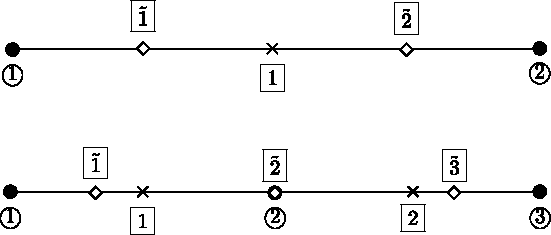
\includegraphics[scale=1]{reduced_integration_tying_points.pdf}
\caption{The tying points used to alleviate membrane and transverse shear locking are defined based on reduced integration quadrature.}
\end{figure}


Figure 1 shows a finite element, across which linear shape functions $N_1$ and $N_2$ are associated with nodes \textcircled{1} and \textcircled{2}. Also, it shows a constant shape function $\bar{N}_1$ defined over the element, associated with a tying point \fbox{1}. The shape functions $N_1$ and $N_2$ are of order one (i.e. $p=1$), and they are defined over an element of two nodes (i.e. $n_e = p+1 = 1+1 = 2$). The shape function $\bar{N}_1$, however, is associated with the tying point \fbox{1}, defined by a one-order lower Gaussian quadrature. Thus, the shape function $\bar{N}_1$ is of order zero (i.e. $\bar{p} = p-1 = 1-1 = 0$). The relationships $n_t = n_e -1$ and $\bar{p} = p - 1$, hold.

\begin{figure}[hbt!]
\centering
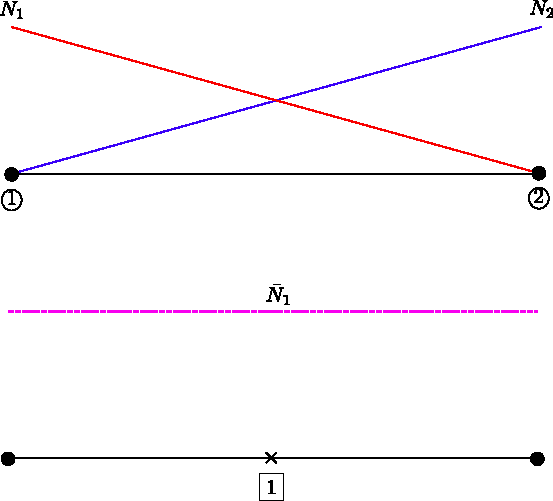
\includegraphics[scale=1]{linear_shape_functions_vs_tying_point.pdf}
\caption{The linear shape functions $N_1$ and $N_2$ associated with the nodes (above) and shape function $\bar{N}_1$ associated with the tying point (below).}
\end{figure}

Similarly, Figure 2 shows a finite element, over which quadratic shape functions $N_1$, $N_2$ and $N_3$ are associated with nodes \textcircled{1}, \textcircled{2} and \textcircled{3}. Moreover, it shows linear shape functions $\bar{N}_1$ and $\bar{N}_2$ defined over the element, associated with tying points \fbox{1} and \fbox{2}. The shape functions $N_1$, $N_2$ and $N_3$ are of order two (i.e. $p=2$), and they are defined over an element of three nodes (i.e. $n_e = p+1 = 2+1 = 3$). The shape functions $\bar{N}_1$ and $\bar{N}_2$, however, are of order one (i.e. $\bar{p} = p-1 = 2-1 = 1$).


\begin{figure}[hbt!]
\centering
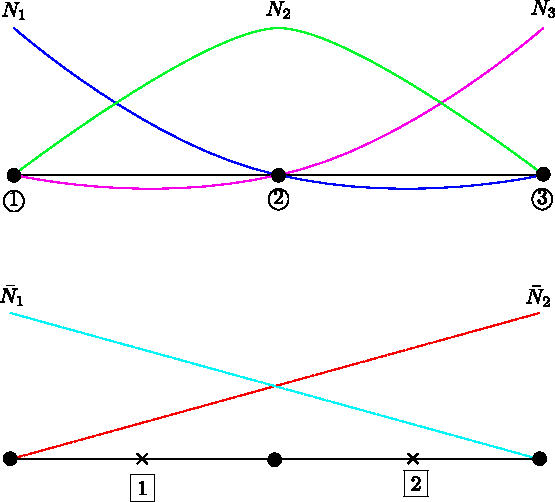
\includegraphics[scale=1]{quadratic_shape_functions_vs_tying_point}
\caption{The quadratic shape functions $N_1$, $N_2$ and $N_3$ associated with the nodes (above) and shape functions $\bar{N}_1$ and $\bar{N}_2$ associated with the tying points (below).}
\end{figure}

It can be seen that the interpolatory property holds for the shape functions $N_I$ at the nodes. That is, $N_I(\xi_J) = \delta_{IJ}$. However, this property does not hold for the shape functions $\bar{N}_I$ at the tying points. 

After the tying points are defined as described above, the method detailed in Section 1 is used to obtain the strain-displacement matrix modified with ANS, $\text{\bf{B}}^{\text{ANS}}$. Rows one, four and six from the standard compatible strain-displacement matrix, $\text{\bf{B}}$, have to be replaced accordingly.







\section{ANS for Alleviating Curvature-Thickness Locking}

Curvature-thickness locking leads to activating spurious transverse normal strains. Accordingly, the strain components in $\eta \eta$ and $\zeta \zeta$ directions have to be modified via replacing the second and third rows of the standard compatible strain-displacement matrix, $\text{\bf{B}}$, with what is obtained from the matrix modified using ANS, $\text{\bf{B}}^{\text{ANS}}$.

Following the work of many researchers, since the prastatic terms vanish at nodal points, the assumed natural strain (ANS) method interpolates the transverse normal strains at nodes. For instance, for a linear brick element, in $\xi$-direction, the tying points are chosen to be at the edges of the element. When the brick element is nonlinear in the direction of $\xi$, the inner tying points occur at equidistant distances. In $\eta$ and $\zeta$ directions, however, the points corresponding to full Gaussian integration are used.


In Figure 4, a linear and a quadratic elements are represented. The equidistant nodes are denoted with black circles. The diamonds show the integration points based on a full Gaussian quadrature. The tying points are coincident with the nodes and also equidistant.

\begin{figure}[hbt!]
\centering
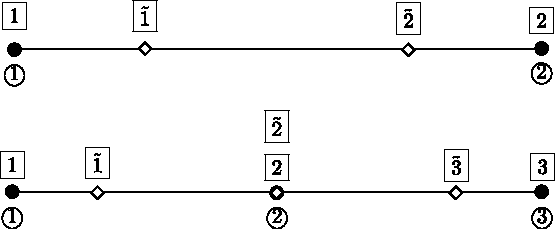
\includegraphics[scale=1]{coincident_tying_points_curvature_locking.pdf}
\caption{The tying points used to alleviate curvature-thickness locking are defined to be coincident with the nodes.}
\end{figure}

Here, the number of tying points, $n_t$, is equal to the number of nodes, $n_e$. The shape functions that are used to interpolate the strains, $\bar{N}_I$, are identical to those used to interpolate the displacements, $N_I$, as the tying points coincide with the nodes. $\boldsymbol{M}$ reduces to an identity matrix because the shape functions are interplatory here.


\section{Modifying the Geometric Stiffness Matrix}

As the strain-displacement matrix is modified, the geometric part of the stiffness matrix needs to be adjusted accordingly. Recall that the geometric part of the stiffness matrix is given by:

\begin{equation}
\boldsymbol{K}^g_{IJ} = \int_{\Omega_\square} S_{IJ} \boldsymbol{I}_3 J^e \ \mathrm{d}\xi \mathrm{d}\eta \mathrm{d}\zeta,
\end{equation}

\noindent
where $I,J \in \{1, 2, \cdots, n_e \}$ and $S_{IJ}$ is given by:

\begin{equation}
S_{IJ} := \begin{bmatrix}
N_{I,\xi} & N_{I,\eta} & N_{I,\zeta}  \\
\end{bmatrix}
\begin{bmatrix}
S_{\xi\xi} & S_{\xi\eta} & S_{\xi\zeta}  \\
S_{\eta\xi} & S_{\eta\eta} & S_{\eta\zeta}  \\
S_{\zeta\xi} & S_{\zeta\eta} & S_{\zeta\zeta}  \\
\end{bmatrix}
\begin{bmatrix}
N_{J,\xi}  \\
N_{J,\eta}  \\
N_{J,\zeta}  \\
\end{bmatrix}.
\end{equation}

Expanding Equation (14) yields:

\begin{equation}
\begin{split}
S_{IJ} = N_{I,\xi} S_{\xi \xi} N_{J,\xi} + N_{I,\xi} S_{\xi \eta} N_{J,\eta} + N_{I,\xi} S_{\xi \zeta} N_{J,\zeta} \\ + N_{I,\eta} S_{\eta \xi} N_{J,\xi} + N_{I,\eta} S_{\eta \eta} N_{J,\eta} + N_{I,\eta} S_{\eta \zeta} N_{J,\zeta} \\ + N_{I,\zeta} S_{\zeta \xi} N_{J,\xi} + N_{I,\zeta} S_{\zeta \eta} N_{J,\eta} + N_{I,\zeta} S_{\zeta \zeta} N_{J,\zeta},
\end{split}
\end{equation}

\noindent
which demonstrates that $\boldsymbol{K}^g_{IJ}$ can be additively decomposed into nine components, as follows:

\begin{equation}
\begin{split}
\boldsymbol{K}^g_{IJ} = \prescript{}{\xi \xi}{\boldsymbol{K}}^g_{IJ} + \prescript{}{\xi \eta}{\boldsymbol{K}}^g_{IJ} + \prescript{}{\xi \zeta}{\boldsymbol{K}}^g_{IJ} \\
+ \prescript{}{\eta \xi}{\boldsymbol{K}}^g_{IJ} + \prescript{}{\eta \eta}{\boldsymbol{K}}^g_{IJ} + \prescript{}{\eta \zeta}{\boldsymbol{K}}^g_{IJ} \\
+ \prescript{}{\zeta \xi}{\boldsymbol{K}}^g_{IJ} + \prescript{}{\zeta \eta}{\boldsymbol{K}}^g_{IJ} + \prescript{}{\zeta \zeta}{\boldsymbol{K}}^g_{IJ}.
\end{split}
\end{equation}

As ANS method is not applied for the strain components in $\eta \zeta$ and $\zeta \eta$, the contributions  $\prescript{}{\eta \zeta}{\boldsymbol{K}}^g_{IJ}$ and $\prescript{}{\zeta \eta}{\boldsymbol{K}}^g_{IJ}$ do not need to be modified, and thus are given by:

\begin{subequations}
\begin{eqnarray}
\prescript{}{\eta \zeta}{\boldsymbol{K}}^g_{IJ} = \int_{\Omega_\square} N_{I,\eta} S_{\eta \zeta} N_{J,\zeta} \boldsymbol{I}_3 J^e \ \mathrm{d}\xi \mathrm{d}\eta \mathrm{d}\zeta, \\
\prescript{}{\zeta \eta}{\boldsymbol{K}}^g_{IJ} = \int_{\Omega_\square} N_{I,\zeta} S_{\zeta \eta} N_{J,\eta} \boldsymbol{I}_3 J^e \ \mathrm{d}\xi \mathrm{d}\eta \mathrm{d}\zeta.
\end{eqnarray}
\end{subequations}

For all the other contributions, the expressions must be modified due to the application of ANS method. That is,

\begin{subequations}
\begin{eqnarray}
\prescript{}{\xi \xi}{\boldsymbol{K}}^g_{IJ} = \int_{\Omega_\square} S_{\xi \xi} (N_{I,\xi}  N_{J,\xi})^* \boldsymbol{I}_3 J^e \ \mathrm{d}\xi \mathrm{d}\eta \mathrm{d}\zeta, \\
\prescript{}{\xi \eta}{\boldsymbol{K}}^g_{IJ} = \int_{\Omega_\square} S_{\xi \eta} (N_{I,\xi}  N_{J,\eta})^* \boldsymbol{I}_3 J^e \ \mathrm{d}\xi \mathrm{d}\eta \mathrm{d}\zeta, \\
\prescript{}{\xi \zeta}{\boldsymbol{K}}^g_{IJ} = \int_{\Omega_\square} S_{\xi \zeta} (N_{I,\xi}  N_{J,\zeta})^* \boldsymbol{I}_3 J^e \ \mathrm{d}\xi \mathrm{d}\eta \mathrm{d}\zeta, \\
\prescript{}{\eta \xi}{\boldsymbol{K}}^g_{IJ} = \int_{\Omega_\square} S_{\eta \xi} (N_{I,\eta}  N_{J,\xi})^* \boldsymbol{I}_3 J^e \ \mathrm{d}\xi \mathrm{d}\eta \mathrm{d}\zeta, \\
\prescript{}{\eta \eta}{\boldsymbol{K}}^g_{IJ} = \int_{\Omega_\square} S_{\eta \eta} (N_{I,\eta}  N_{J,\eta})^* \boldsymbol{I}_3 J^e \ \mathrm{d}\xi \mathrm{d}\eta \mathrm{d}\zeta, \\
\prescript{}{\zeta \xi}{\boldsymbol{K}}^g_{IJ} = \int_{\Omega_\square} S_{\zeta \xi} (N_{I,\zeta}  N_{J,\xi})^* \boldsymbol{I}_3 J^e \ \mathrm{d}\xi \mathrm{d}\eta \mathrm{d}\zeta, \\
\prescript{}{\zeta \zeta}{\boldsymbol{K}}^g_{IJ} = \int_{\Omega_\square} S_{\zeta \zeta} (N_{I,\zeta}  N_{J,\zeta})^* \boldsymbol{I}_3 J^e \ \mathrm{d}\xi \mathrm{d}\eta \mathrm{d}\zeta.
\end{eqnarray}
\end{subequations}


In general, one can write:

\begin{equation}
(N_{I,K}  N_{J,L})^* = 
\begin{bmatrix}
\bar{N}_1 (\xi) & \bar{N}_2 (\xi) & \cdots & \bar{N}_{n_t} (\xi)
\end{bmatrix}_{(1 \times n_t)} \boldsymbol{M}^{-1}_{(n_t \times n_t)}
\begin{bmatrix}
N_{I,K}(\hat{\xi}_1,\eta,\zeta) N_{J,L}(\hat{\xi}_1,\eta,\zeta) \\
N_{I,K}(\hat{\xi}_2,\eta,\zeta) N_{J,L}(\hat{\xi}_2,\eta,\zeta) \\
  \vdots \\
N_{I,K}(\hat{\xi}_{n_t},\eta,\zeta) N_{J,L}(\hat{\xi}_{n_t},\eta,\zeta)
\end{bmatrix}_{(n_t \times 1)},
\end{equation}

\noindent
where $K,L \in \{\xi,\eta,\zeta \}$.

It is noteworthy that none of the expressions given in Equations (17) and (18) are generally symmetric. Equation (19) is applied on contributions $\eta \eta$ and $\zeta \zeta$ slightly differently than the other contributions because they are associated with different tying points.


\section{Overall Implementation Algorithm}

The procedure discussed here to alleviate locking is performed entirely at the element level, which makes it easier to implement in existing codes.

\begin{algorithm}
\caption{Calculation of the material and geometric parts of an element tangent stiffness matrix, and element internal force vectors, using the Assumed Natural Strain method (ANS)}\label{alg:cap}
\LinesNumbered
\textbf{Input:} Initial geometry of the element, nodal displacements, material properties;\\
\textbf{Result:} Material and geometric parts of element tangent stiffness matrix, $\boldsymbol{K}^m_e$ and $\boldsymbol{K}^g_e$, and element internal force vector, $\boldsymbol{f}_{int}^e$;\\
\For{$every\text{ }Gauss\text{ }point\text{ }in\text{ }the\text{ }e^{th}\text{ }element$}
{
	Start as in standard formulation;\\
	Calculate the standard compatible strain-displacement matrix $\text{\bf{B}}$ at Gauss integration points;\\
	\For{$every\text{ }tying\text{ }point\text{ }to\text{ }alleviate\text{ }membrane\text{ }and\text{ }transverse\text{ }shear\text{ } locking$}
	{
	Calculate $\boldsymbol{N}$ based on $\bar{N}$ shape functions and the integration point coordinates;\\
	Calculate $\boldsymbol{M}$ based on $\bar{N}$ shape functions and the tying point coordinates;\\
	Calculate the first, fourth and sixth lines of the standard compatible strain-displacement matrix, $\text{\bf{B}}$, at the tying points;\\


	}
	Calculate the first, fourth and sixth lines of the ANS modified strain-displacement matrix, $\text{\bf{B}}^{\text{ANS}}$, at the integration points;\\
	Replace the first, fourth and sixth lines of $\text{\bf{B}}$ by those of $\text{\bf{B}}^{\text{ANS}}$;\\

	
		\For{$every\text{ }tying\text{ }point\text{ }to\text{ }alleviate\text{ }curvature\text{ }locking$}
	{
	Calculate $\boldsymbol{N}$ based on $\bar{N}$ shape functions and the integration point coordinates;\\
	Calculate $\boldsymbol{M}$ based on $\bar{N}$ shape functions and the tying point coordinates;\\
	Calculate the second and third lines of the standard compatible strain-displacement matrix, $\text{\bf{B}}$, at the tying points;\\

	}
	Calculate the second and third lines of the ANS modified strain-displacement matrix, $\text{\bf{B}}^{\text{ANS}}$, at the integration points;\\
	Replace the second and third lines of $\text{\bf{B}}$ by those of $\text{\bf{B}}^{\text{ANS}}$;\\
	Internal force vector and material stiffness matrix using $\text{\bf{B}}^{\text{ANS}}$;\\
		\For{$every\text{ }node\text{ }in\text{ }the\text{ }e^{th}\text{ }element$}
	{
	Calculate all contributions of the geometric stiffness matrix using Equations (17) and (18);\\
	}

	Add all contributions of the geometric stiffness matrix;\\

}
	Add the material and geometric parts of the the stiffness matrix;
\end{algorithm}





\end{document}
